

\chapter{Rabi Oscillations}



\section{Tasks}

\begin{itemize}
\item  Visualize the  path of the Bloch vector and its components when a laser pulse shines on a two-level system. Use a numerical method to integrate the differential equation. Investigate both resonant and non-resonant cases.
\end{itemize}



\section{Experiment}

Many experimental realizations show Rabi oscillations. We will discuss them in term of a two-level system interacting with an optical field, for example an atom in vacuum or a molecule or quantum dot in solid state at low temperature. But the same description holds also for many other systems. In fact, a two-level system is equivalent to a spin $1/2$ system, as an electron spin or nuclear spin. The same concepts are thus applied in electron spin resonance or nuclear magnetic resonance experiments (ESR and NMR).

We shine a laser beam on an atom, molecule, quantum dot. The laser frequency is close the the optical transition. We measure the populations of the excited state by, e.g. fluorescence emission or tunneling of the electron out of this state. We switch on the laser for a given time duration $t$ and measure the signal amplitude as function of $t$. This a little bit indirect experiment is necessary, as $t$ is in many cases short to the emission or tunneling rate. Only in theory we can measure the population of the state while it is evolving. We find periodic oscillations of the signal amplitude, the Rabi oscillations.\sidenote{needs papers!}

\section{Density Matrix}


We start by introducing the density matrix.\footcite{Rand2016,Parson,Hamm-dummies}
It is a tool in quantum mechanics to describe not only purely coherent states, but also statistical mixtures, as we will see below. The density matrix is a bit at the edge of the classical canon of quantum mechanics lectures.

When  writing our wave function $\ket{\psi}$ in  a basis $\ket{n}$ as
\[
 \ket{\psi} = \sum_n c_n \, \ket{n}
\]
then we can define a density operator $\hat{\rho}$ as
\[
\hat{\rho} =  \ket{\rho}\bra{\rho} = \sum_{m,n} c_n c_m^\star \, \ket{n}\bra{m}
\]
and the matrix elements of $\boldsymbol{\rho}$ are $\rho_{m,n} =  c_n c_m^\star$. The density matrix allows to calculate the expectation value of any operator $\hat{A}$ as
\[
 \braket{\hat{A}} =  \braket{\psi | \hat{A} | \psi}  = \sum_{m,n} c_n c_m^\star \, A_{m,n} = \sum_{m,n} \rho_{n,m} \,  \, A_{m,n} = Tr ( A \rho)
\]
where the trace sums over the diagonal elements
\[
 Tr (U ) = \sum_n U_{n,n}  \quad .
\]
The trace of the density matrix is one for normalized states 
\[
 Tr (\rho) = \sum_n \rho_{n,n} = \sum_n c_n c_n^\star = 1 \quad \text{if normalized}
\]
The interesting thing comes when looking at pure and mixed states. Pure states are the 'conventional' states discussed in quantum mechanics, for example this superposition of states
\[
\ket{\psi} = \sqrt{\frac{1}{2}} \left( \ket{1} + \ket{2} \right) 
\]
In this example, the density matrix reads
\[
 \rho = \frac{1}{2} \begin{pmatrix}
 1 & 1 \\ 1 & 1 \\
 \end{pmatrix}
\]
and its trace is one. But the density matrix also allows to describe new things, beyond pure states, namely statistical mixtures of states. We can describe an ensemble of two-level systems, of which half the ensemble is in state $\ket{1}$, the other half in state $\ket{2}$. This can \emph{not} be written as 
$\ket{1} + \ket{2} $, but a density matrix description is possible as
\[
 \rho = \frac{1}{2} \begin{pmatrix}
 1 & 0 \\ 0 & 1 \\
 \end{pmatrix} \quad .
\]
The diagonal elements of the density matrix describe the populations of the states, i.e. $|c_n|^2$. The off-diagonal elements describe coherence between states. In a statistical mixture there is no coherence between the states, as one sub-ensemble is in one state, another in another state, and they don't know anything of each other.

We can distinguish between pure and mixed states by looking at the trace of the squared density matrix
\begin{eqnarray*}
 Tr (\rho^2) & = & 1 \quad \text{pure state} \\
 				& < & 1 \quad \text{mixed state} \\
\end{eqnarray*}

Mixed states can be  used not only to describe an ensemble of systems in different states, but also to describe a single system that at different times is in different states. Even if we can do an experiment on  a single quantum system, we have to repeat it very often to reduce noise by averaging. But the experiment does not always run along the same path: either a photon is absorbed or not, but it will most likely not \emph{always}  we absorbed. The time-average of such an experiment will thus need  an statistical mixture for its description.

\section{Liouville--von Neumann equation}

We can construct a differential equation for the time evolution of the density matrix that is a direct analogue of the Schrodinger equation, just that is also takes mixed states into account.

The time-derivative of the density matrix $\rho$ is
\[
 \frac{d}{dt} \rho = \frac{d}{dt} \left( \ket{\psi} \bra{\psi} \right) 
 =  \left( \frac{d}{dt}  \ket{\psi} \right) \bra{\psi} 
 + \ket{\psi} \left( \frac{d}{dt}  \bra{\psi} \right) 
\]
Making use of the Schrodinger equation
\[
 \frac{d}{dt} \ket{\psi} = - \frac{i}{\hbar} \, \hat{H} \, \ket{\psi}
\]
we get the Liouville--von Neumann equation
\[
 \frac{d}{dt} \rho = - \frac{i}{\hbar} 
 \left[ \hat{H} , \rho \right]  \quad .
\]

As an example, let us look at a two-level system with the eigen-energies $E_0= 0$ and $E_1 = \hbar \omega_0$. The Hamilton operator is thus
\[
 \hat{H } = \begin{pmatrix}
  0 & 0 \\ 0 & \hbar \omega_0 \\
 \end{pmatrix}
\]
The commutator becomes
\[
 \left[ \hat{H}, \rho \right] = 
 \begin{pmatrix}
 0 & - \hbar \omega_0 \, \rho_{01} \\   \hbar \omega_0 \, \rho_{10} & 0 \\
 \end{pmatrix}
\]
The  diagonal elements of the density matrix $\rho$, i.e., the populations, remain thus constant in time, as expected for this Hamiltonian. The off-diagonal elements, the coherences acquire a phase-factor proportional to the energy difference, i.e.
\[
 \rho_{01}(t) =  \rho_{01}(0) \, \exp \left(i \, \omega_0 \, t \right) 
\]

\section{Optical Bloch Equations}

Now we switch on light and add an interaction Hamiltonian $\hat{H}_I = -\boldsymbol{\mu} \, \boldsymbol{E}$ of dipole operator $\boldsymbol{\mu} $ and optical field   $\boldsymbol{E}$. In total, the Hamilton operator reads\footcite[chap. 3.8]{Rand2016}
\[
 \hat{H } = \begin{pmatrix}
  0 & - {\boldsymbol{\mu}} \, \boldsymbol{E} \\ - {\boldsymbol{\mu}}^\star \, \boldsymbol{E}^\star & \hbar \omega_0 \\
 \end{pmatrix}
\]
The differential equations for the density matrix become the Bloch equations
\begin{eqnarray*}
\dot{\rho}_{00} &=&  - \frac{i}{\hbar} \left( \rho_{10} \boldsymbol{\mu} \, \boldsymbol{E} - \rho_{01} \boldsymbol{\mu}^\star \, \boldsymbol{E}^\star \right) \\
%
\dot{\rho}_{11} &=&  - \frac{i}{\hbar} \left( \rho_{01} \boldsymbol{\mu} \, \boldsymbol{E} - \rho_{10} \boldsymbol{\mu}^\star \, \boldsymbol{E}^\star \right) \\
%
\dot{\rho}_{01} &=& - \frac{i}{\hbar}  \left( - \rho_{01} \hbar \omega_0 + (\rho_{00} - \rho_{11})  \boldsymbol{\mu} \, \boldsymbol{E} \right) \\
%
\dot{\rho}_{10} &=& - \frac{i}{\hbar}  \left( + \rho_{10} \hbar \omega_0 + (\rho_{11} - \rho_{00})  \boldsymbol{\mu}^\star \, \boldsymbol{E}^\star \right) \\
\end{eqnarray*}
We can simplify things by skipping some algebraic transformations and introducing the Bloch\sidenote{The physics of two-level systems is always the same. This formalism also applies to spin-1/2 systems like electron spins or nuclear spins in ESR and NMR experiments.} vector $\boldsymbol{a}$ with
\[
\boldsymbol{a} = 
\begin{pmatrix}
u \\ v \\ w \\
\end{pmatrix}
= 
\begin{pmatrix}
\rho_{10} + \rho_{01} \\ i (\rho_{10} - \rho_{01}) \\ \rho_{00} - \rho_{11} \\
\end{pmatrix}
= 
\begin{pmatrix}
\Re (\rho_{10})  \\ \Im (\rho_{10}) \\ \rho_{00} - \rho_{11} \\
\end{pmatrix}
\]
With this we can write the system of differential equation as 
\[
 \dot{\boldsymbol{a}} = \boldsymbol{M}   \times \boldsymbol{a} 
 \quad \text{with} \quad 
 \boldsymbol{M}  = 
 \begin{pmatrix}
 \frac{2}{\hbar} \, \Re ( \boldsymbol{\mu} \, \boldsymbol{E} ) \\
  \frac{2}{\hbar} \, \Im ( \boldsymbol{\mu} \, \boldsymbol{E} ) \\
  \omega_0
 \end{pmatrix}
\]
The time evolution of the Bloch vector, and by this of the density matrix, can be described by the action of a torque vector $\boldsymbol{M}$. Without optical field, the Bloch vector rotates around its $w$ axis, as seen in the phase oscillation of the coherences in the last chapter. With optical field, also the populations changes, and things become complicated.

To simplify things, we assume that our optical field is a single mode with a slowly varying amplitude only, i.e.
\[
 \boldsymbol{E}(t) = \boldsymbol{x} \, E_0(t) \left( e^{i \omega_L t} + e^{-i \omega_L t} \right)
\]
The time-dependence of $E(t)$ should be slow compared to $\omega_L t$. This is the slowly-varying amplitude approximation (SVEA). Then we move into a rotating frame. Our new coordinate system rotates around the $w$ axis with the angular frequency of the laser $\omega_L$. The optical frequency of the transition $\omega_0$ is close to this laser frequency. We neglect terms of $\omega_0 + \omega_L$ and only keep terms of  $\omega_0 - \omega_L$. The first will oscillate fast and average out, the latter oscillate slowly. This is the rotating wave approximation (RWA). In total we get in the rotating frame 
\[
 \dot{\boldsymbol{a}'} = \boldsymbol{M}'   \times \boldsymbol{a}' 
 \quad \text{with} \quad 
 \boldsymbol{M}'  = 
 \begin{pmatrix}
2 \mu    |E(t)| / \hbar \\
0 \\
\omega_0 - \omega_L
 \end{pmatrix} = 
  \begin{pmatrix}
\Omega \\
0 \\
\omega_0 - \omega_L
 \end{pmatrix}
\]
with the (angular) Rabi frequency $\hbar \Omega = 2 \mu    |E(t)| $ and $\mu = \boldsymbol{\mu \, x}$ the project of the transition dipole moment on the polarization direction of the light field. In the following, we stay in the rotating frame and leave out the prime symbols.


\section{Rabi Oscillations}

Let us discuss the time evolution of the Bloch vector in the rotating frame. Applying only a torque $\boldsymbol{M}$, the length of the Bloch vector does not change. It moves along the surface of a sphere, the Bloch sphere. The sphere has a diameter of one when the density matrix describes a normalized pure state. For mixed states, the Bloch vector is shorter. Below we will see how dephasing and relaxation processes reduce the length of the Bloch vector.


A two-level system in the ground state is on the north pole of the sphere. The state $\ket{0} + \ket{1}$ is on the equator, pointing along the $u$ axis. All points except the poles contain a coherence between the two levels.


\begin{figure}
\caption{Some Bloch vectors and their positions on the Bloch sphere.}
\end{figure}


The torque $\boldsymbol{M}$ rotates the Bloch vector around  $\boldsymbol{M}$ with a angular frequency  $|\boldsymbol{M}|$. A resonant laser field, i.e., $\omega_L = \omega_0$ rotates the Bloch vector around the $u$ axis. When this field acts continuously, the Bloch vector moves from the north pole via the equator to the south pole and back to the north pole and so on. The population of the states changes periodically from zero to one:
\[
 \rho_{00} = \cos ( \Omega \, t)^2 \quad .
\]
These are the Rabi oscillations. When the laser is not fully resonant, the Bloch vector rotates around an axis in the $u$-$w$ plane. Starting from the ground state at the north pole, it thus does not reach the south pole any more. The population of the excited state will  not reach one.

\begin{figure} 
    \centering
    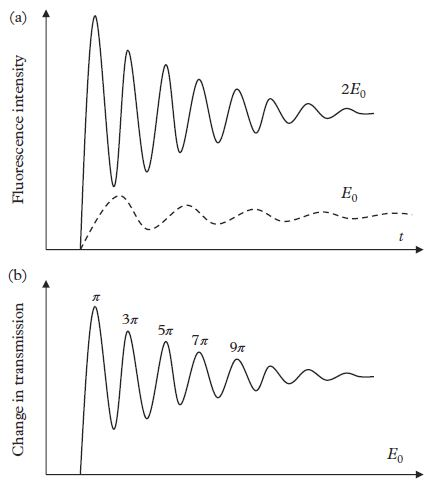
\includegraphics[width = 0.7 \textwidth]{\currfiledir/Rabi1.JPG}
    \caption{Rabi oscillations in (a) transient fluorescence and (b) differential transmission.}
    \label{fig:Rabi}
\end{figure}

We can observe these oscillations by any method that can determine the population of the excited state, for example fluorescence emission, electron emission or (transient) absorption.


** Introduce pulse area


\section{Damping and dephasing}


\begin{align*}
    i\hbar \dot{\hat{\rho}} =& [\hat{H},\hat{\rho}] + \text{relaxation}
     \notag\\
    =& [\hat{H},\hat{\rho}] \pm i\hbar\Lambda \pm i\hbar\gamma \hat{\rho} - i\hbar \Gamma \hat{\rho}
\end{align*}


The first term takes into account the decrease due to incoherent pumping, the second the radiative and non-radiative population relaxation. The last one considers dephasing. 





\printbibliography[segment=\therefsegment,heading=subbibliography]
